\documentclass[a4paper,10pt]{article}

\usepackage{graphicx}
\usepackage{amsmath}
\usepackage[spanish]{babel}
\usepackage[utf8]{inputenc} % Permite escribir directamente áéíóúñ
\usepackage[hidelinks]{hyperref}
\usepackage{pdfpages}

\title{ \textbf{ 6620. Organizaci\'on de Computadoras\\
Trabajo Pr\'actico 1: \\
Conjunto de instrucciones MIPS}}

\author{ Riesgo, Daniela, \textit{Padr\'on Nro. 95557} \\
\texttt{ danielap.riesgo@gmail.com } \\[2.5ex]
Martin, D\'ebora, \textit{Padr\'on Nro. 90934} \\
\texttt{ debbie1mes.world@gmail.com } \\[2.5ex]
Constantino, Guillermo, \textit{Padr\'on Nro. 89776} \\
\texttt{ guilleconstantino@gmail.com } \\[2.5ex]
\normalsize{2do. Cuatrimestre de 2014} \\
\normalsize{66.20 Organizaci\'on de Computadoras $-$ Pr\'atica Martes} \\
\normalsize{Facultad de Ingenier\'ia, Universidad de Buenos Aires} \\
}

\date{}

\begin{document}
\maketitle
\thispagestyle{empty} % quita el nmero en la primer pagina

\begin{abstract}
El presente trabajo tiene como objetivo familiarizarse con el conjunto de instrucciones MIPS y el concepto de ABI, extendiendo un programa escrito en C que resuelva el problema del conjunto de Multibrot de orden 3, ocupándose de la funci\'on que calcula la velocidad de escape e imprime en el archivo de la salida lo correspondiente.

\end{abstract}

\cleardoublepage
\setcounter{page}{0}
\newpage
\tableofcontents
\newpage
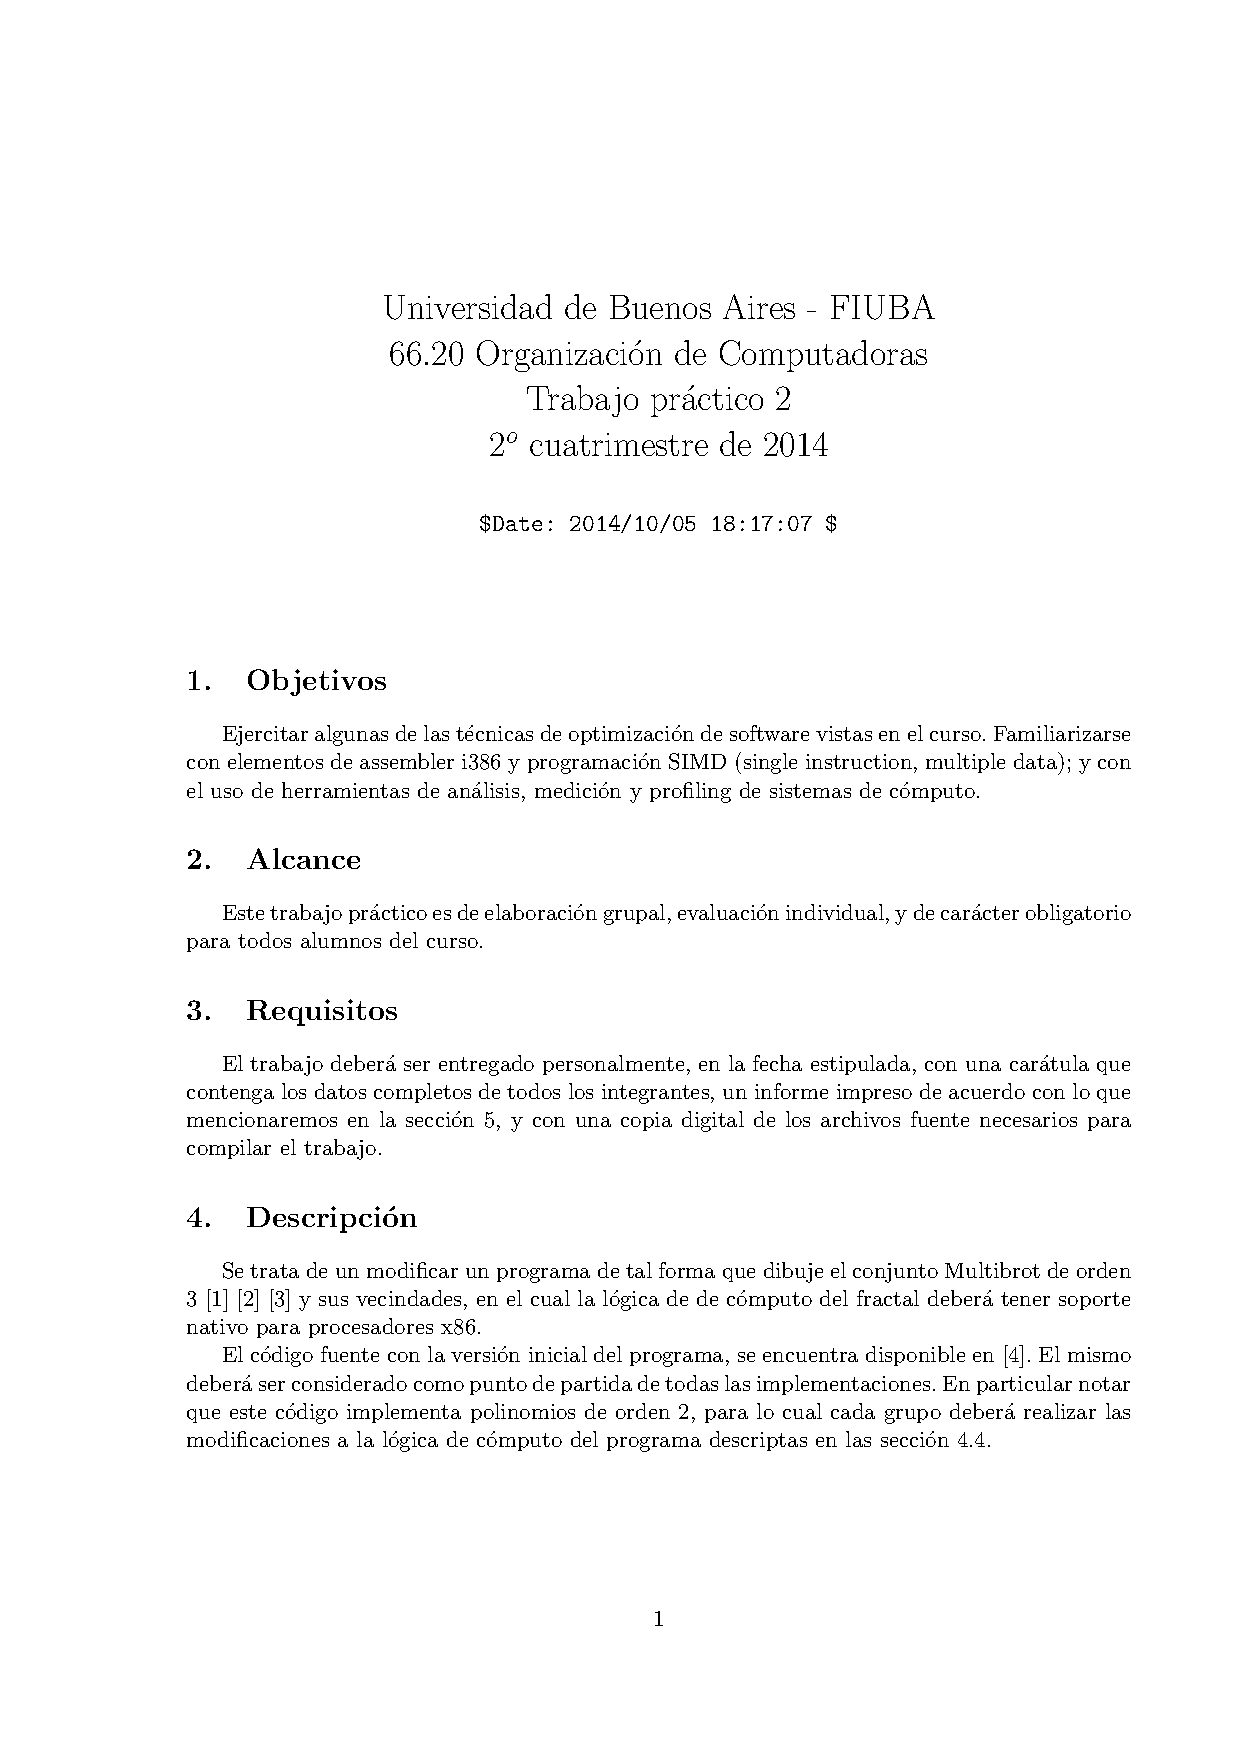
\includepdf[pages={-}, pagecommand={\thispagestyle{empty}}, addtotoc={1, section, 1, Enunciado, enunciado}]{./Enunciado.pdf}

\section{Introducci\'on}
Al comenzar a utilizar nuevas herramientas, en cualquier \'ambito, es necesaria una breve introducci\'on al funcionamiento de las mismas: tener una noci\'on de las prestaciones que ofrecen, asi tambi\'en como de sus limitaciones.\\
En este trabajo pr\'actico continuamos con las nuevas herramientas, esta vez con el objetivo de 
familiarizarse con el conjunto de instrucciones de MIPS32 a partir de una arguitectura NetBSD/pmax.
De esta forma se pueden reforzar conocimientos como el alineamiento de datos y descubrir las 
instrucciones y pseudo-instrucciones que MIPS ofrece para trabajar.
Otro aspecto importante del trabajo es la necesidad de trabajar con registros de punto flotante y 
entender c\'omo los registros est\'an en procesadores separados y tienen otras instrucciones propias.




\section{Programa a implementar}
Se trata de, teniendo el programa en C como fuente, implementar una de las funciones, aquella que se encarga 
de dibujar el conjunto de Multibrot de orden 3 y sus vecindades, en lenguaje Assembly para MIPS32 
en NetBSD/pmax.
La misma recibir\'a por par\'ametro una estructura con la informaci\'on definida en la l\'inea de 
comando con la que se ejecuta el programa; información como el centro del plano complejo, la resoluci\'on deseada, entre otras.
Al finalizar la ejecuci\'on y volver al programa, la funci\'on habr\'a escrito en el archivo de salida 
los par\'ametros necesarios y el brillo correspondiente a cada pixel de forma que se genere una imagen con el fractal buscado.
El formato gr\'afico a usar es PGM o portable gray map, un formato simple para describir im\'agenes a
digitales monocrom\'aticas.





\section{Explicaci\'on de la Implementaci\'on}
Este trabajo present\'o varios problemas a resolver. 
Por un lado, la escritura en un archivo. Se aprendi\'o que la estructura FILE hace referencia a un 
descriptor de archivo \'unico e intr\'inseco a cada archivo, necesario para escribir en el archivo. 
Este n\'umero ocupa menos de una palabra y entonces debi\'o alinearse usando la instrucci\'on 
prove\'ida por MIPS para cargar media palabra. 
También relacionado a la escritura, un desaf\'io fue convertir n\'umeros contenidos en registros en 
cadenas de caracteres. Para esto se us\'o como gu\'ia un ejercicio similar hecho en clase. 
Por otro lado, se resolvieron las cuentas propiamente dicha manejando registros e instrucciones. 
Finalmente se tuvo que manejar tanto los registros y su contenido como el frame de la funci\'on, 
respetando las convenciones ABI y descifrando los tamaños de las distintas secciones del frame seg\'un 
cu\'anta informaci\'on era necesaria descargar en el frame.
Finalmente el frame qued\'o distribuido de la siguiente forma:

\begin{itemize}


\begin{center}
\begin{tabular}{ r | p{1cm} | c | l }
  \cline{2-2}              
   & & & \\        
   & SRA & & \\ 
   & & & \\ \cline{2-2}
   & & & \\ 
   & LTA & &  56 \\ 
   & & & \\ \cline{2-2}
   & & & \\ 
   & ABA & &\\
   & & & \\ 
  \cline{2-2}
\end{tabular}
\end{center}


\item \textbf{SRA}
\begin{center}
\begin{tabular}{ r | c | c | l }
  \cline{2-2}                       
  52 & Padd& & \\ \cline{2-2}
  48 & ra & &  16 \\ \cline{2-2}
  44 & fp& & \\ \cline{2-2}
  40 & sp & &\\
  \cline{2-2}
\end{tabular}
\end{center}

\item \textbf{LTA}
\begin{center}
\begin{tabular}{ r | c | c | l }
  \cline{2-2}                       
  36 &Padd& & \\ \cline{2-2}
  32 & vel & &   \\ \cline{2-2}
  28 & res\_x & & 24 \\ \cline{2-2}
  24 & x & &\\ \cline{2-2}
  20 & res\_y & & \\ \cline{2-2}
  16 & y & &\\
  \cline{2-2}
\end{tabular}
\end{center}

\item \textbf{ABA}
\begin{center}
\begin{tabular}{ r | p{1cm} | c | l }
  \cline{2-2}                       
  12 &  & & \\ \cline{2-2}
  8 &   & &  16 \\ \cline{2-2}
  4 &  & & \\ \cline{2-2}
  0 &   & &\\
  \cline{2-2}
\end{tabular}
\end{center}


\end{itemize}



\section{C\'odigo assembly}
Para generar el ejecutable del programa se utiliz\'o el makefile prove\'ido de forma que se tome 
el c\'odigo de $mips32__plot.S$ en vez de $mips32__plot.c$. 
Para tratar la impresi\'on de strings, se decidi\'o copiar el c\'odigo necesario cada vez que se quer\'ia 
imprimir porque no ocupaba m\'as de 8 l\'ineas de c\'odigo. A diferencia de la transformaci\'on 
necesaria de n\'umero a cadena que se requer\'ia en varias oportunidades que levaba bastantes l\'ineas m\'as. 
Se trat\'o de usar etiquetas que identifiquen las partes de la funci\'on, constantes que expliciten la interpretaci\'on de un simple n\'umero y comentarios que expliquen 
el significado de las instrucciones usadas.
Tambi\'en se trat\'o de minimizar la transferencia de datos y por lo tanto se trat\'o de manejar el 
procesamiento \'unicamente con los registros temporales, sin dar uso no necesario a la LTA. 


\pagebreak




\section{Corridas de prueba}

Como en este trabajo s\'olo se deb\'ia programar la parte de dibujo del fractal, los casos de prueba 
no testean la interfaz. Simplemente hicimos uso de las dos im\'agenes prove\'idas para saber c\'omo 
deb\'ia resultar la imagen y probar el programa.\\

1. Generamos la imagen por defecto, es decir, barriendo el rect\'angulo de plano complejo desde 
-0.65 + 0.30i hasta -0.55 + 0.20i:
\begin{verbatim}
> tp1-2014-2-bin -o uno.pgm
\end{verbatim}

\begin{figure}
\begin{center}

\includegraphics[width=0.8\textwidth]{./uno.pgm}
\label{fig:Region barrida por defecto.}
\caption{}
\end{center}
\end{figure}


2. En este caso generamos una imagen que comprenda desde -0.625 + 0.625i hasta -0.575 + 0.575i:
\begin{verbatim}
> tp1-2014-2-bin --center -0.6+0.6i --width 0.05 --height 0.05 -o dos.pgm
\end{verbatim}

\begin{figure}
\begin{center}
\includegraphics[width=0.8\textwidth]{./dos.pgm}
\label{fig:Region comprendida entre -0.625+0.625i y -0.575+0.575i.}
\caption{}
\end{center}
\end{figure}

3. Imagen imposible:
\begin{verbatim}
> ./tp0 -c 0+0i -r 0x1 -o -
COMPLETAAAAAAAR !
\end{verbatim}

4. Archivo de salida imposible:
\begin{verbatim}
> ./tp0 -o /tmp
COMPLETAAAAAAAR !
\end{verbatim}

5. Coordenadas complejas imposibles:
\begin{verbatim}
> ./tp0 -c 1+3 -o -
COMPLETAAAAAAAR !
\end{verbatim}

6. Generamos una imagen de 1 punto de lado, centrada en el or\'igen del plano complejo:
\begin{verbatim}
> ./tp0 -c 0+0i -r 1x1 -o -
VERIFICAR RESULTADO !!!! COPIAR TEXTUALMENTE
P2
1
1
255
255
\end{verbatim}

Notar que el resultado es correcto, ya que este punto pertenece al conjunto de Multibrot de orden 3.\\
\\

7. Repetimos el experimento, pero nos centramos ahora en un punto que seguro no pertenece
al conjunto:
\begin{verbatim}
> ./tp0 -c 10+0i -r 1x1 -o -
VERIFICAR RESULTADO !!!! COPIAR TEXTUALMENTE
P2
1
1
255
0
\end{verbatim}

Notar que el resultado es correcto, ya que este punto pertenece al conjunto de Multibrot de orden 3.
\\



\section{C\'odigo fuente C}

\begin{verbatim}
#include <mips/regdef.h>
#include <sys/syscall.h>
.abicalls

.text
.align 2

.global mips32_plot
.ent mips32_plot

mips32_plot:

FRAME_SPACE = 56
.frame $fp, FRAME_SPACE, ra
subu sp, sp, FRAME_SPACE # Pongo el stack pointer al final de mi frame.
.cprestore 40?  ?  # El gp en 40(sp)
sw $fp, 44(sp)
sw ra, 48(sp)

#Pongo el frame pointer al final de mi frame.
or $fp, sp, zero

# Información de datos
LARGO_NUM = 1
LARGO_P2 = 3
LARGO_ENTER = 1
LARGO_IO_ERROR = 11

#Offset dentro de la estructura param.
OFF_UPPER_LEFT_REAL = 0?  ?  ?  #float: 1 registro f
OFF_UPPER_LEFT_IMAG = 4 ?  ?  ?  #float: 1 registro f
OFF_LOWER_RIGHT_REAL = 8 ?  ?  ?  #float: 1 registro f
OFF_LOWER_RIGHT_IMAG = 12 ?  ?  #float: 1 registro f
OFF_SCALE_REAL = 16 ?  ?  ?  ?  #float: 1 registro f
OFF_SCALE_IMAG = 20 ?  ?  ?  ?  #float: 1 registro f
OFF_RES_REAL = 24 ?  ?  ?  ?  #size_t = unsigned: 1 registros
OFF_RES_IMAG = 28 ?  ?  ?  ?  #size_t = unsigned: 1 registros
OFF_SHADES = 32 ?  ?  ?  ?  ?  #size_t = unsigned: 1 registros
OFF_OUTPUT_FILE = 36 ?  ?  ?  ?  #puntero: 1 registro
#Offset del numero de archivo dentro de la estructura _sFile
OFF_FILE_NUMBER = 14 ?  ?  ?  #short int: 1/2 registro


sw a0, FRAME_SPACE($fp)

l.s $f0, OFF_UPPER_LEFT_IMAG(a0) # F0 para upper_left_im
l.s $f2, OFF_SCALE_IMAG(a0) # F2 para d_im

l.s $f6, OFF_UPPER_LEFT_REAL(a0) # F6 para upper_left_re
l.s $f8, OFF_SCALE_REAL(a0) # F8 para d_re

lw t6, OFF_OUTPUT_FILE(a0)
lh t6, OFF_FILE_NUMBER(t6) # T6 para el file descriptor.

imprimir_p2:
?  li v0, SYS_write
?  move a0, t6
?  la a1, p2
?  li a2, LARGO_P2
?  syscall
?  # Si me devolvió un número no nulo en a3, hubo error.
?  bne a3, zero, imprimir_io_error
  ?  blt v0, a2, imprimir_io_error
?  lw a0, FRAME_SPACE($fp) #recargo a0 con la estructura porque en el 
?  # imprimir se pisa

imprimir_res_x:
?  lw t8, OFF_RES_REAL(a0)
?  la t9, imprimir_res_y
?  j imprimir_numero
?  lw a0, FRAME_SPACE($fp)
?  
imprimir_res_y:
?  lw t8, OFF_RES_IMAG(a0)
?  la t9, imprimir_max_gray
?  j imprimir_numero
?  lw a0, FRAME_SPACE($fp)
?  
imprimir_max_gray:
?  lw t8, OFF_SHADES(a0)
?  la t9, empezar
?  j imprimir_numero
?  lw a0, FRAME_SPACE($fp)

empezar:
?  li t0, 0 ?  ?  ?  ?  # T0 es y
?  lw t1, OFF_RES_IMAG(a0) # T1 res_y
?  mov.s $f4, $f0 ?  ?  ?  # F4 copia del up_im para ir modificando (ci)
?  li t2, 0 ?  ?  ?  ?  # T2 para x
?  lw t3, OFF_RES_REAL(a0) # T3 para res_x
?  mov.s $f10, $f6 ?  ?  # F10 copia del up_re (cr)
?  li t4, 0 ?  ?  ?  ?  # T4 para la velocidad de escape.
?  lw t5, OFF_SHADES(a0)?  # T5 para el máximo de grises

loop_vertical:
?  beq t0, t1, terminar # Si y llegó a ser el último pixel, termino.
?  loop_horizontal:
?  ?  beq t2, t3, aumento_loop_vert

?  ?  mov.s $f12, $f4 # F12 guarda la copia del ci (zi)
?  ?  mov.s $f14, $f10 # F14 guarda la copia del cr (zr)

?  ?  loop_mandelbrot:
?  ?  ?  beq t4, t5, imprimir_brillo

?  ?  ?  # Calculo el módulo
?  ?  ?  mul.s $f16, $f12, $f12 # F16 guarda zi*zi
?  ?  ?  mul.s $f18, $f14, $f14 # F18 guarda zr*zr
?  ?  ?  add.s $f20, $f16, $f18 # F20 guarda zi*zi+zr*zr
?  ?  ?  li.s $f22, 4.0 # F22 guarda 4
?  ?  ?  c.lt.s $f22, $f20 # Si F22<F20 pone el flag en true.
?  ?  ?  bc1t imprimir_brillo # Va a imprimir brillo si el flag es false, es decir,
?  ?  ?  # si el módulo es mayor a 4.

?  ?  ?  mul.s $f20, $f12, $f16 # F20 guarda zi*zi*zi
?  ?  ?  mul.s $f22, $f14, $f18 # F22 guarda zr*zr*zr
?  ?  ?  mul.s $f24, $f16, $f14 # F24 guarda zi*zi*zr
?  ?  ?  mul.s $f26, $f18, $f12 # F26 guarda zr*zr*zi
?  ?  ?  li.s $f28, 3.0 # F28 guarda 3
?  ?  ?  mul.s $f24, $f28, $f24 # F12 guarda 3*zi*zi*zr
?  ?  ?  mul.s $f26, $f28, $f26 # F26 guarda 3*zr*zr*zi
?  ?  ?  sub.s $f22, $f22, $f24 # F22 guarda zr*zr*zr - 3*zi*zi*zr
?  ?  ?  add.s $f22, $f22, $f4 # F22 guarda sr
?  ?  ?  sub.s $f26, $f26, $f20 # F26 guarda 3*zr*zr*zi - zi*zi*zi
?  ?  ?  add.s $f26, $f26, $f10 # F26 guarda si
?  ?  ?  mov.s $f12, $f26
?  ?  ?  mov.s $f14, $f22

?  ?  ?  add t4, t4, 1 # Aumento la velocidad de escape en 1
?  ?  ?  j loop_mandelbrot

?  ?  imprimir_brillo:
?  OFF_FRAME_Y = 16
?  OFF_FRAME_RES_Y = 20
?  OFF_FRAME_X = 24
?  OFF_FRAME_RES_X = 28
?  OFF_FRAME_VEL = 32
?  ?  guardar:?  
?  ?  ?  sw t0, OFF_FRAME_Y($fp)
?  ?  ?  sw t1, OFF_FRAME_RES_Y($fp)
?  ?  ?  sw t2, OFF_FRAME_X($fp)
?  ?  ?  sw t3, OFF_FRAME_RES_X($fp)
?  ?  ?  sw t4, OFF_FRAME_VEL($fp)
?  ?  ?  
?  ?  ?  move t8, t4
?  ?  ?  la t9, recargar
?  ?  ?  j imprimir_numero
?  ?  
?  ?  recargar:
?  ?  ?  lw t0, OFF_FRAME_Y($fp)
?  ?  ?  lw t1, OFF_FRAME_RES_Y($fp)
?  ?  ?  lw t2, OFF_FRAME_X($fp)
?  ?  ?  lw t3, OFF_FRAME_RES_X($fp)
?  ?  ?  lw t4, OFF_FRAME_VEL($fp)

?  aumento_loop_hor:
?  ?  add t2, t2, 1 ?  ?  # Aumento x en 1.
?  ?  add.s $f10, $f10, $f8 ?  # Aumento cr según la escala.
?  ?  j loop_horizontal
aumento_loop_vert:
?  add t0, t0, 1 ?  ?  # Aumento y en 1.
?  sub.s $f4, $f4, $f2 ?  # A ci le resto según la escala.
?  j loop_vertical


terminar:
?  lw ra, 32($fp)
?  lw gp, 24($fp)
?  lw $fp, 28($fp)
?  addu sp, sp, FRAME_SPACE
?  jr ra

MAX_DIV = 100?  ?  # Es el máximo divisor de acuerdo a la cantidad máxima de 
# cifras que puede tener el número a imprimir.

imprimir_numero:?  # Recibe registros T6, T8 (y lo cambia) y T9; usa
# registros T0, T1, T2, T3 y T4
# T6 es el archivo donde debo imprimir.
# T8 tiene el número de 3 cifras máximo.
# T9 tiene a donde debo volver para seguir ejecutando el programa.
?  li t0, MAX_DIV?  ?  # T0 para el divisor.
?  imp_cifra:
?  ?  beq t0, 0, volver?  # Si ya imprimió todo, vuelve al programa.
?  ?  divu t1, t8, t0?  ?  # T1 para el cociente de num/div
?  ?  rem t2, t8, t0?  ?  # T2 para el resto de num/div
?  escribir_num:
?  ?  # El número a imprimir está en T1
?  ?  la t3, numeros?  ?  # T3 para la dirección del arreglo.
?  ?  # La posición en el arreglo es número por 4 (ya que cada palabra son 4 bytes).
?  ?  sll t4, t1, 2?  ?  # T4 tiene la poscición del número en el arreglo.
?  ?  addu t4, t3, t4?  ?  # T4 tiene la dirección donde está la dirección de la
?  ?  # etiqueta del número.
?  ?  lw t4, 0(t4)?  ?  # T4 tiene dirección de la etiqueta del número.
?  ?  
?  ?  li v0, SYS_write
?  ?  move a0, t6
?  ?  lw a1, 0(t4)
?  ?  li a2, LARGO_NUM
?  ?  syscall
?  ?  # Si me devolvió un número no nulo en a3, hubo error.
?  ?  bne a3, zero, imprimir_io_error
?  ?  blt v0, a2, imprimir_io_error
?  ?  
?  proximo:
?  ?  move t8, t2
?  ?  divu t0, t0, 10?  ?  # Para testear la siguiente cifra.
?  ?  j imp_cifra
?  
?  volver:
    # Imprimo un enter.
    li v0, SYS_write
?  ?   move a0, t6
?  ?  la a1, enter
?  ?  li a2, LARGO_ENTER
?  ?  syscall
?  ?  # Si me devolvió un número no nulo en a3, hubo error.
?  ?  bne a3, zero, imprimir_io_error
    blt v0, a2, imprimir_io_error
?  ?  
    jr t9


STD_ERR = 2?  ?  
imprimir_io_error:
?  li v0, SYS_write
?  li a0, STD_ERR
?  la a1, error_io
?  li a2, LARGO_IO_ERROR
?  syscall
?  j exit

exit:
?  li v0, SYS_exit
?  syscall


.end mips32_plot


.rdata

p2: .asciiz "P2\n"

.align 2

numeros: .word cero, uno, dos, tres, cuatro, cinco, seis, siete, ocho, nueve
cero: .ascii "0"
uno: .ascii "1"
dos: .ascii "2"
tres: .ascii "3"
cuatro: .ascii "4"
cinco: .ascii "5"
seis: .ascii "6"
siete: .ascii "7"
ocho: .ascii "8"
nueve: .ascii "9"


enter: .asciiz "\n"

error_io: .asciiz "i/o error.\n"

\end{verbatim}

\pagebreak



\section{Conclusiones}
El trabajo pr\'activo motivo de este informe ha presentado al equipo diversos desaf\'ios. 
Estos  desaf\'ios llevaron a familiarizarse con las instrucciones que provee MIPS32, de forma 
de conocer los recursos que se tienen para resolver un problema y entender la arquitectura de 
los procesadores. Por otro lado, se reforz\'o el uso de las convenciones de ABI para manejar las 
llamadas a funciones; aunque la programada no llamaba a otra funci\'on, s\'i deb\'ia respetar a la 
funci\'on que la hab\'ia llamado.
Por las razones expuestas, consideramos muy \'util| un trabajo pr\'actico introductorio de esta 
naturaleza para empezar a conocer las utilidades del lenguaje y arquitectura estudiados.\\

\pagebreak

\begin{thebibliography}{99}

\bibitem{GXEMUL} GXemul, \url{http://gxemul.sourceforge.net/}

\bibitem{NETBSD} The NetBSD Project, \url{http://www.netbsd.org/}

\bibitem{PGMFORMAT} PGM format specification.
\url{http://netpbm.sourceforge.net/doc/pgm.html}

\bibitem{LATEX} Oetiker, Tobias, "The Not So Short Introduction To LaTeX2", \url{http://www.physics.udel.edu/$\sim$dubois/lshort2e/}

\end{thebibliography}


\end{document}